\documentclass{article}


\usepackage[a4paper]{geometry}
\usepackage{pgfplots}
\pgfplotsset{compat=1.9}


\usepackage{parskip}


\usepackage[justification=centering]{caption}
\usepackage{subcaption}
\usepackage{graphicx}
\usepackage{float}
\usepackage{amsmath}
\usepackage{booktabs}
\usepackage{tabularx}
\usepackage{perpage}
\usepackage{smartdiagram}
\usepackage{cancel}
\usepackage{amssymb}
\usepackage{bm}
\usepackage{longtable}
\usepackage{listings}
\usepackage{courier}
\usepackage{fancybox}
\newcolumntype{P}[1]{>{\centering\arraybackslash}p{#1}}
\usepackage{hhline}
\usepackage{bm}
\usepackage{siunitx}
\usepackage[utf8]{inputenc}
\usepackage[english]{babel}
\usepackage{graphicx}
\usepackage{amsthm}
\usepackage{tabularray}
\usepackage{verbatim}
\usepackage{verbatimbox}
\usepackage{array}
\usepackage{ulem}
\usepackage{mathtools}
\usepackage{amsfonts}

\usepackage{color}

\usepackage{xparse}




\usepackage{tikz}
\usetikzlibrary{calc}
\usetikzlibrary{automata}
\usetikzlibrary{backgrounds}
\usetikzlibrary{fit}
\usetikzlibrary{arrows}
\usetikzlibrary{arrows.meta}
\usetikzlibrary{decorations.pathreplacing}
\usetikzlibrary{decorations.markings}
\usetikzlibrary{positioning}
\usetikzlibrary{intersections}
\usetikzlibrary{calligraphy}
\usetikzlibrary{patterns}
\usetikzlibrary{shapes}
\usetikzlibrary{shapes.geometric}
\usetikzlibrary{shadows}
\usetikzlibrary{fadings}
\usetikzlibrary{backgrounds}
\usepgflibrary{shadings}
\usepgfplotslibrary{colorbrewer}
\pgfplotsset{cycle list/Blues-9}

\tikzset{
    loop above right/.style={above right, out= 60, in= 30, loop},
    loop above left/.style ={above left,  out=150, in=120, loop},
    loop below right/.style={below right, out=330, in=300, loop},
    loop below left/.style ={below left,  out=240, in=210, loop}
}

\tikzset{%
  show curve controls/.style={
        postaction={
            decoration={
                show path construction,
                curveto code={
                \draw [blue] 
                    (\tikzinputsegmentfirst) -- (\tikzinputsegmentsupporta)
                    (\tikzinputsegmentlast) -- (\tikzinputsegmentsupportb);
                \fill [red, opacity=0.5] 
                    (\tikzinputsegmentsupporta) circle [radius=.5ex]
                    (\tikzinputsegmentsupportb) circle [radius=.5ex];
                }
            },
            decorate
        }
    }
}

\renewcommand{\thefootnote}{\fnsymbol{footnote}}
\MakePerPage{footnote}


\newtheorem{theorem}{Theorem}[section]
\newtheorem*{theorem*}{Theorem}
\newtheorem{corollary}{Corollary}[theorem]
\newtheorem*{corollary*}{Corollary}
\newtheorem{lemma}[theorem]{Lemma}
\newtheorem*{lemma*}{Lemma}


\newtheorem*{claim}{Claim}

\theoremstyle{definition}
\newtheorem*{proposition}{Proposition}

\theoremstyle{definition}
\newtheorem{definition}{Definition}[section]

\theoremstyle{remark}
\newtheorem*{remark}{Remark}
\newtheorem*{example}{Example}
\newtheorem*{exercise}{Exercise}

\renewcommand\qedsymbol{$\blacksquare$}

\usepackage[myheadings]{fullpage}
\usepackage{fancyhdr}
\usepackage{lastpage}
\usepackage{float}
\usepackage{url}
\usepackage{lipsum}
\usepackage[T1]{fontenc}
\usepackage{icomma}
\usepackage{siunitx}
\usepackage{ragged2e}
\usepackage{comment}
\usepackage{multicol}
\usepackage{caption}
\usepackage{float}
\usepackage{titling}
\usepackage{blindtext}
\usepackage{mathdots}
\usepackage{enumitem}
\usepackage{adjustbox}
\usepackage{colortbl}

\pagestyle{fancy}
%\renewcommand{\chaptername}{}
%\renewcommand{\chaptermark}[1]{\markboth{#1}{}}
\renewcommand{\sectionmark}[1]{\markright{#1}{}}
%\renewcommand{\subsectionmark}[1]{\markright{#1}{}}

\fancyhf{}
\setlength\headheight{15pt}
\fancyhead[L]{Tikz/PGF} %>>>MODULE CODE
\fancyhead[R]{reeeeeee} %>>>MODULE NAME
\fancyfoot[C]{Bottom text | \thepage}

\fancypagestyle{plain}{%
    \fancyhf{}%
    \renewcommand{\headrulewidth}{0pt}% 
}

\frenchspacing
\usepackage{bigfoot}
\renewcommand{\footnoterule}{\vfill\kern -3pt \hrule width 0.4\columnwidth \kern 2.6pt}

\usepackage{comment}

\newcommand{\Tikz}{Ti\textit{k}z{}}


\title{Introduction to PGF/\Tikz{}}
\author{Kit Liu}

\begin{document}

\maketitle

\vspace{1cm}

\begin{center}
    
\begin{tikzpicture}
        \filldraw[draw=none, fill=black, opacity=0.65]
            (1.9,0.1) ellipse (2.9 and 0.7);
        \path[save path=\back]
            {[rounded corners=15pt]
            (0,5)
         -- (-1,5)
         -- (-1,1.5)}
         -- (0,1.5)
         -- cycle;
        \filldraw[red, use path=\back];
        \begin{scope}
            \clip[use path=\back];
            \filldraw[draw=none, fill=purple, opacity=0.95]
                {[rounded corners=5pt]
                (-1,4.1)
             -- (-0.5,4)}
             -- (0,4.1)
             -- (0,1.5)
             -- (-1,1.5)
             -- cycle;
        \end{scope}
        \draw[line width=4mm, use path=\back, draw=black];
        \path[save path=\body]
            {[rounded corners=15pt]
            (0,3)
         -- (0.15,0)
         -- (1.7,0)}
            {[rounded corners=5pt]
         -- (1.75,1.5)
         -- (3,1.5)}
         -- (2.35,1.5)
            {[rounded corners=15pt]
         -- (2.4,0.25)
         -- (3.9,0.25)}
            {[rounded corners=15pt]
         -- (4,1.4)
         -- (4.2,2.5)}
            {[rounded corners=45pt]
         -- (3.9,6.8)
         -- (0.15,7)
         -- cycle};
        \filldraw[red, use path=\body];
        \begin{scope}
            \clip[use path=\body];
            \filldraw[draw=none, fill=purple, opacity=0.95]
                (0,9)
             -- (1,7)
                {[rounded corners=40pt]
             -- (0.4,6)
             -- (0.8,2)
             -- (4,2)}
             -- (4,4.5)
             -- (4,0)
             -- (0,0)
             -- cycle;
        \end{scope}
        \draw[line width=4mm, use path=\body, draw=black];
        \draw[rounded corners=25pt, fill=cyan!40!white, draw=black]
            (4.5,6) rectangle (1.5,4);
        \begin{scope}
            \clip (4.5,6) [rounded corners=25pt] rectangle (1.5,4);
            \filldraw[draw=none, fill=blue!50!black, opacity=0.5]
                {[rounded corners=20pt]
                (2.1,6.2)
             -- (2.1,4.7)
             -- (4.6,4.7)}
             -- (4.6,5.2)
             -- (4.6,4)
             -- (1.5,4)
             -- (1.5,6)
                {[rounded corners=20pt]
             -- (2.5,6)
             -- cycle};
            \draw[very thick, rounded corners=7.5pt, fill=white!90, draw=none]
                (4,5.5) rectangle (2.8,5);
        \end{scope}
        \draw[rounded corners=25pt, line width=4mm, draw=black]
            (4.5,5.9) rectangle (1.5,4);
    \end{tikzpicture}
\end{center}




\begin{verbbox}[\small]

\begin{tikzpicture}
    \filldraw[draw=none, fill=black, opacity=0.65]
        (1.9,0.1) ellipse (2.9 and 0.7);
    \path[save path=\back]
        {[rounded corners=15pt]
        (0,5)
     -- (-1,5)
     -- (-1,1.5)}
     -- (0,1.5)
     -- cycle;
    \filldraw[red, use path=\back];
    \begin{scope}
        \clip[use path=\back];
        \filldraw[draw=none, fill=purple, opacity=0.95]
            {[rounded corners=5pt]
            (-1,4.1)
         -- (-0.5,4)}
         -- (0,4.1)
         -- (0,1.5)
         -- (-1,1.5)
         -- cycle;
    \end{scope}
    \draw[line width=4mm, use path=\back, draw=black];
    \path[save path=\body]
        {[rounded corners=15pt]
        (0,3)
     -- (0.15,0)
     -- (1.7,0)}
        {[rounded corners=5pt]
     -- (1.75,1.5)
     -- (3,1.5)}
     -- (2.35,1.5)
        {[rounded corners=15pt]
     -- (2.4,0.25)
     -- (3.9,0.25)}
        {[rounded corners=15pt]
     -- (4,1.4)
     -- (4.2,2.5)}
        {[rounded corners=45pt]
     -- (3.9,6.8)
     -- (0.15,7)
     -- cycle};
    \filldraw[red, use path=\body];
    \begin{scope}
        \clip[use path=\body];
        \filldraw[draw=none, fill=purple, opacity=0.95]
            (0,9)
         -- (1,7)
            {[rounded corners=40pt]
         -- (0.4,6)
         -- (0.8,2)
         -- (4,2)}
         -- (4,4.5)
         -- (4,0)
         -- (0,0)
         -- cycle;
    \end{scope}
    \draw[line width=4mm, use path=\body, draw=black];
    \draw[rounded corners=25pt, fill=cyan!40!white, draw=black]
        (4.5,6) rectangle (1.5,4);
    \begin{scope}
        \clip (4.5,6) [rounded corners=25pt] rectangle (1.5,4);
        \filldraw[draw=none, fill=blue!50!black, opacity=0.5]
            {[rounded corners=20pt]
            (2.1,6.2)
         -- (2.1,4.7)
         -- (4.6,4.7)}
         -- (4.6,5.2)
         -- (4.6,4)
         -- (1.5,4)
         -- (1.5,6)
            {[rounded corners=20pt]
         -- (2.5,6)
         -- cycle};
        \draw[very thick, rounded corners=7.5pt, fill=white!90, draw=none]
            (4,5.5) rectangle (2.8,5);
    \end{scope}
    \draw[rounded corners=25pt, line width=4mm, draw=black]
        (4.5,5.9) rectangle (1.5,4);
\end{tikzpicture}
\end{verbbox}


\scalebox{0.8}{\theverbbox}

\newpage

\section*{What is PGF/\Tikz{}?}

PGF/\Tikz{} is a pair of languages for generating \textit{vector graphics}. That is, graphics constructed from geometric primitives (points/vertices, line segments, polyhedra, parametric surfaces, etc.), with each primitive assigned a set of properties (colour, line weight, dash patterns, etc.). This is in contrast to \textit{raster graphics}, in which each pixel of the image is stored (e.g. with colour, luminance, transparency values, etc.).

Because vector graphics consist of coordinates/lines/curves, the size of a representation on a screen is independent of the size of the object -- you can zoom in to a vector image arbitrarily close and it will remain crisp.

Furthermore, the parameters of vector objects can be later modified, so that moving, scaling, rotating, filling, etc. does not degrade the quality of a vector image. In contrast, repeated modifications to a raster image will continually degrade the image quality as elements are snapped to a pixel grid between each edit.

\section*{Getting Started}

A \Tikz{} diagram is built within the \verb|tikzpicture| environment. Primitives are specified and drawn using \Tikz{} commands within the environment, each terminated with a semicolon (\verb|;|).

% Here is an example of some \Tikz{} code, and its output:

\subsection*{Specifying Points}

There are many ways to specify \textit{points} or \textit{coordinates} in \Tikz{}. Coordinates are always written with round brackets.

You can declare your coordinate system explicitly (this will be more relevant later) with the syntax
\begin{verbatim}
    ([coordinate system] cs: (system-specific coordinates))
\end{verbatim}
but for various common coordinate systems, special implicit syntax is available.

For instance, cartesian coordinate may be specified explicitly using the \verb|canvas| coordinate system:
\begin{verbatim}
    (canvas cs:x=2ex,y=5pt)
\end{verbatim}
which takes two keys, \verb|x| and \verb|y|, that accept \TeX{} dimensions. Or, they can be specified implicitly by listing the two dimensions separated by commas in round brackets, as in
\begin{verbatim}
    (2ex,5pt)
\end{verbatim}
This coordinate means ``2ex upwards and 5pt to the right of the origin''.

Note that, with the \verb|calc| library loaded, you can also write things like \verb|1em+2cm| in a dimension, since the maths engine is used to evaluate the coordinates.

\begin{verbbox}[\small\mbox{}]
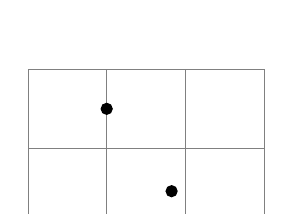
\begin{tikzpicture}
    \draw[help lines] (0,0) grid (3,2);

    \filldraw (1cm,1.5cm)   circle (2pt);
    \filldraw (2cm-5pt,3ex) circle (2pt);
\end{tikzpicture}
\end{verbbox}
\begin{center}
    $\vcenter{\hbox{
    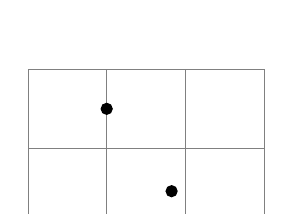
\begin{tikzpicture}
        \draw[help lines] (0,0) grid (3,2);
    
        \filldraw (1cm,1.5cm)   circle (2pt);
        \filldraw (2cm-5pt,3ex) circle (2pt);
    \end{tikzpicture}
    }}$
    \hspace*{0.5cm}
    $\vcenter{\hbox{\theverbbox}}$
\end{center}

Polar coordinates may be specified using the \verb|canvas polar| system
\begin{verbatim}
    (canvas polar cs:angle=30,radius=2cm)
\end{verbatim}
or implicitly by providing the angle and a radius separated by a colon:
\begin{verbatim}
    (30:2cm)
\end{verbatim}
This coordinate means ``2cm from the origin, 30 degrees counterclockwise from the positive $x$-axis''.

\begin{verbbox}[\small\mbox{}]
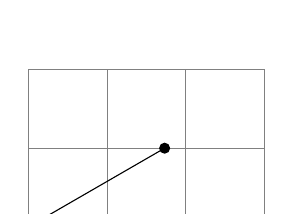
\begin{tikzpicture}
    \draw[help lines] (0,0) grid (3,2);
    \draw (0,0) -- (30:2cm);

    \fill (30:2cm) circle (2pt);
\end{tikzpicture}
\end{verbbox}
\begin{center}
    $\vcenter{\hbox{
    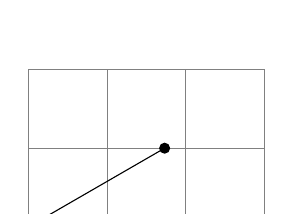
\begin{tikzpicture}
        \draw[help lines] (0,0) grid (3,2);
        \draw (0,0) -- (30:2cm);
    
        \fill (30:2cm) circle (2pt);
    \end{tikzpicture}
    }}$
    \hspace*{0.5cm}
    $\vcenter{\hbox{\theverbbox}}$
\end{center}

There are other coordinate systems, but I'll only expand more on those on request. From now on, we'll also omit the explicit system declaration unless it is otherwise relevant.

If units are not provided, e.g. \verb|(1,2)|, then the coordinates are specified in PGF's internal \verb|xy|-coordinate system. By default, the unit $x$-vector points 1cm to the right, and the unit $y$-vector points 1cm upwards.\footnote{It is possible to use coordinates like \verb|(1,2cm)|, which is neither an \verb|xy|-coordinate nor a \verb|canvas| coordinate. Roughly speaking, if you have mixed coordinates, \Tikz{} will typecast the coordinate \verb|(X,Ycm)| to the sum \verb|(X,0)+(0pt,Y)|, and similarly for any mixed dimensions. In particular, \verb|(2+3cm,0)| is \textit{not} the same as \verb|(2cm+3cm,0)|, as it will be typecast to the sum \verb|(2pt,0) + (3cm,0) = (2pt+3cm,0)|.}

By giving three numbers, as in \verb|(1,2,3)|, the coordinates are specified in PGF's internal $xyz$-coordinate system. By default, the unit $x$-vector points 1cm to the right, and the unit $y$-vector points 1cm upwards, and the unit $z$-vector points to \verb|(-3.85mm,-3.85mm)|.

It is also possible to use an anchor (explained later) of an existing shape as in \verb|(my\_node.centre)| as a coordinate.

You can add two plus signs before a coordinate to specify a coordinate relative to the previously defined coordinate. For example, \verb|(1,0) ++(1,0) ++(0,1)| specifies the three coordinates \verb|(1,0)|, then \verb|(2,0)|[=(1,0)+(1,0)], and \verb|(2,1)|[$=(2,0)+(0,1)$].

Instead of two plus signs, you can also add a single one. This also specifies a point in a relative manner, but doesn't update the reference coordinate. For example, \verb|(1,0) +(1,0) +(0,1)| specifies the three coordinates \verb|(1,0)|, then \verb|(2,0)|[$=(1,0)+(1,0)$], and \verb|(1,1)|[$=(1,0)+(0,1)$].

A coordinate may also be given a name using the syntax:
\begin{verbatim}
    \coordinate (name) at (coordinate)
\end{verbatim}
This is useful for repeatedly referencing a coordinate later, or for performing computations.


\subsection*{Paths}

A \textit{path} is a series of curves between points, which need not be connected.

To specify a straight line path between two coordinates, put two dashes between the coordinates. For instance,
\begin{verbatim}
    (0,0) -- (0,1) -- (1,1) -- cycle
\end{verbatim}
specifies a trianglar path, with the special \verb|cycle| coordinate \textit{smoothly} closing the path. To see the difference between using \verb|cycle| and simply repeating the first coordinate, consider the following:
\begin{verbbox}[\small\mbox{}]
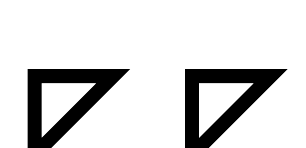
\begin{tikzpicture}[line width=5pt]
    \path[draw] (0,0) -- (0,1) -- (1,1) -- cycle;
    \path[draw] (2,0) -- (2,1) -- (3,1) -- (2,0);
\end{tikzpicture}
\end{verbbox}
\begin{center}
    $\vcenter{\hbox{
    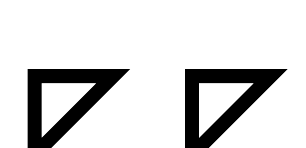
\begin{tikzpicture}[line width=5pt]
        \draw (0,0) -- (0,1) -- (1,1) -- cycle;
        \draw (2,0) -- (2,1) -- (3,1) -- (2,0);
    \end{tikzpicture}
    }}$
    \hspace*{0.5cm}
    $\vcenter{\hbox{\theverbbox}}$
\end{center}

\subsection*{Shapes}

There are various commands for generating predefined shapes and patterns. For instance,
\begin{verbatim}
    (a,b) rectangle (c,d)
\end{verbatim}
specifies a rectangular box with opposite corners at \verb|(a,b)| and \verb|(c,d)|.
\begin{verbbox}[\small\mbox{}]
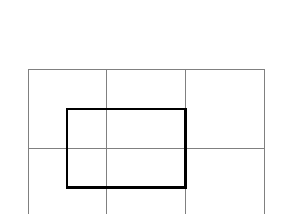
\begin{tikzpicture}[line width=5pt]
    \draw[help lines] (0,0) grid (3,2);

    \draw[thick] (0.5,0.5) rectangle (2,1.5);
\end{tikzpicture}
\end{verbbox}
\begin{center}
    $\vcenter{\hbox{
    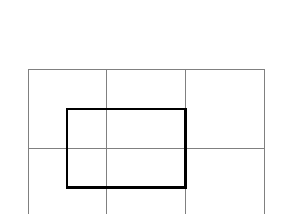
\begin{tikzpicture}
        \draw[help lines] (0,0) grid (3,2);
        
        \draw[thick] (0.5,0.5) rectangle (2,1.5);
    \end{tikzpicture}
    }}$
    \hspace*{0.5cm}
    $\vcenter{\hbox{\theverbbox}}$
\end{center}

\begin{verbatim}
    (a,b) circle (r)
\end{verbatim}
specifies a circle centred at \verb|(a,b)| with radius \verb|r|.
\begin{verbbox}[\small\mbox{}]
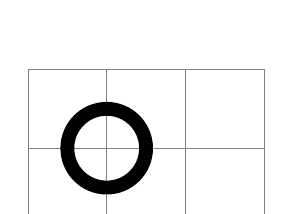
\begin{tikzpicture}[line width=5pt]
    \draw[help lines] (0,0) grid (3,2);
    
    \path[draw] (1,1) circle (0.5);
\end{tikzpicture}
\end{verbbox}
\begin{center}
    $\vcenter{\hbox{
    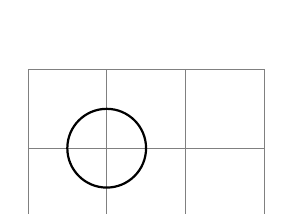
\begin{tikzpicture}
        \draw[help lines] (0,0) grid (3,2);
        
        \draw[thick] (1,1) circle (0.5);
    \end{tikzpicture}
    }}$
    \hspace*{0.5cm}
    $\vcenter{\hbox{\theverbbox}}$
\end{center}


\begin{verbatim}
    (a,b) ellipse [x radius=X, y radius=Y, rotate=T]
\end{verbatim}
specifies an ellipse centred at \verb|(a,b)| with radii \verb|X| and \verb|Y|, and rotation \verb|T|.
\begin{verbbox}[\small\mbox{}]
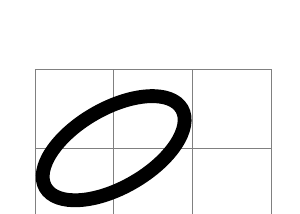
\begin{tikzpicture}[line width=5pt]
    \draw[help lines] (0,0) grid (3,2);
    
    \path[draw] (1,1) ellipse [x radius=1, y radius=0.5, rotate=30];
\end{tikzpicture}
\end{verbbox}
\begin{center}
    $\vcenter{\hbox{
    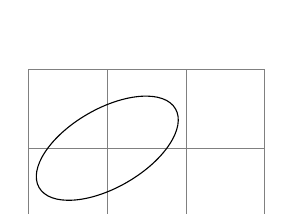
\begin{tikzpicture}
        \draw[help lines] (0,0) grid (3,2);
        
        \path[draw]
            (1,1) ellipse [x radius=1, y radius=0.5,rotate=30];
    \end{tikzpicture}
    }}$
    \hspace*{0.5cm}
    $\vcenter{\hbox{\theverbbox}}$
\end{center}



\subsection*{Arcs}

The \textit{arc} operation draws arcs of ellipses between paths, specified using the following syntax:
\begin{verbatim}
    \path ... arc [radius=R, start angle=A, end angle=B] ... ;
\end{verbatim}
(The $x$ and $y$ radii may also be set separately.)

There also exists a shorter syntax for circular arcs:
\begin{verbatim}
    \path ... arc (start:end:radius) ... ;
\end{verbatim}
However, this form is very difficult to read, so the normal syntax is recommended in general.
\begin{verbbox}[\small\mbox{}]
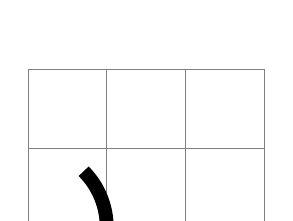
\begin{tikzpicture}[line width=5pt]
    \draw[help lines] (0,0) grid (3,2);
    
    \path[draw] (1,0) arc (0:45:1);
\end{tikzpicture}
\end{verbbox}
\begin{center}
    $\vcenter{\hbox{
    \begin{tikzpicture}
        \draw[help lines] (0,0) grid (3,2);
        
        \path[draw] (1,0) arc (0:45:1);
    \end{tikzpicture}
    }}$
    \hspace*{0.5cm}
    $\vcenter{\hbox{\theverbbox}}$
\end{center}



\subsection*{To}

The \textit{to} operation adds a flexible path between coordinates that may be modified through various options. For instance, there are the \verb|out| and \verb|in| keys, that change the outgoing and incoming angles the path makes to the coordinates:

\begin{verbbox}[\small\mbox{}]
    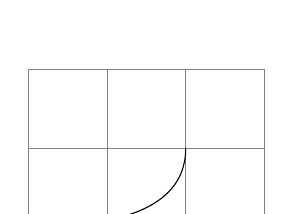
\begin{tikzpicture}
        \draw[help lines] (0,0) grid (3,2);
        
        \path[draw] (0,0) to[out=0,in=-90] (2,1);
    \end{tikzpicture}
\end{verbbox}
\begin{center}
    $\vcenter{\hbox{
    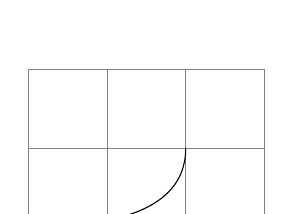
\begin{tikzpicture}
        \draw[help lines] (0,0) grid (3,2);
        
        \path[draw] (0,0) to[out=0,in=-90] (2,1);
    \end{tikzpicture}
    }}$
    \hspace*{0.5cm}
    $\vcenter{\hbox{\theverbbox}}$
\end{center}



\subsection*{Bézier Curves}
Cubic Bézier curves may be specified with the following syntax:
\begin{verbatim}
    \draw (x,y) .. controls (a,b) and (c,d) .. (x,y');
\end{verbatim}
where the coordinates \verb|(a,b)| and \verb|(c,d)| are the two control points of the curve.

\begin{verbbox}[\small\mbox{}]
    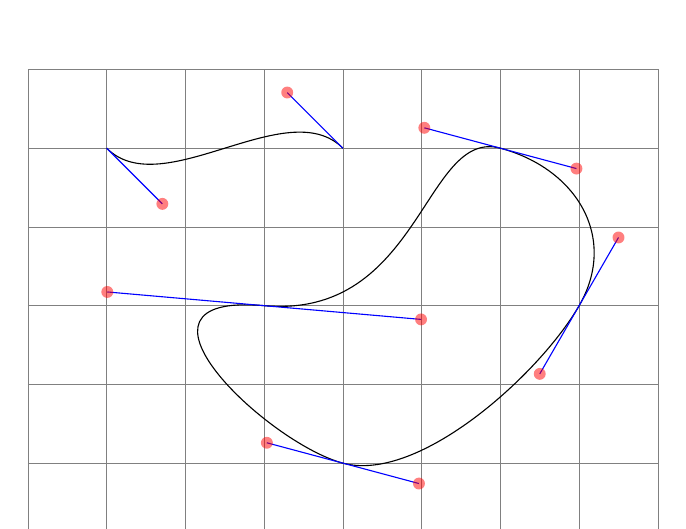
\begin{tikzpicture}
        \draw [help lines] (-4, -1) grid (4, 5);

        \draw [show curve controls]
            (-3, 4) .. controls ++(135:-1) and ++(135:1) .. (0, 4);
        \draw [show curve controls] (0, 0) 
          .. controls ++(165:-1) and ++(240: 1) .. ( 3, 2)
          .. controls ++(240:-1) and ++(165:-1) .. ( 2, 4)
          .. controls ++(165: 1) and ++(175:-2) .. (-1, 2)
          .. controls ++(175: 2) and ++(165: 1) .. ( 0, 0);
    \end{tikzpicture}
\end{verbbox}
\begin{center}
    $\vcenter{\hbox{
    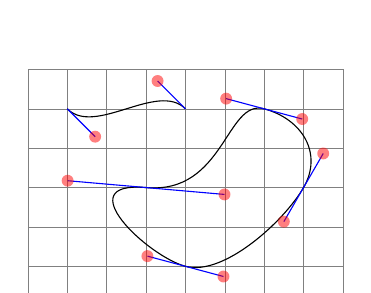
\begin{tikzpicture}[scale = 0.5]
        \draw [help lines] (-4, -1) grid (4, 5);

        \draw [show curve controls]
            (-3, 4) .. controls ++(135:-1) and ++(135:1) .. (0, 4);
        \draw [show curve controls] (0, 0) 
          .. controls ++(165:-1) and ++(240: 1) .. ( 3, 2)
          .. controls ++(240:-1) and ++(165:-1) .. ( 2, 4)
          .. controls ++(165: 1) and ++(175:-2) .. (-1, 2)
          .. controls ++(175: 2) and ++(165: 1) .. ( 0, 0);
    \end{tikzpicture}
    }}$
    \hspace*{5cm}
    $\mathclap{\vcenter{\scalebox{0.75}{\theverbbox}}}$
    \hspace*{5cm}
\end{center}
It is often helpful to specify control points using relative and polar coordinates, as above.


\section*{Actions}

Note that, so far, a path is simply a series of curves and coordinates -- we haven't actually told \Tikz{} what to do with them.

Given a path, we may:
\begin{itemize}
    \item \textit{draw} or \textit{stroke} the path;
    \item \textit{fill} the path;
    \item \textit{clip} the path;
    \item (various other specialised options);
    \item or do any combination of the above.
\end{itemize}

To perform these actions, pass them as options to the \verb|\path| command or use one of these aliases:
\begin{verbatim}
    \draw ...     := \path[draw] ...
    \fill ...     := \path[fill] ...
    \filldraw ... := \path[fill,draw] ...
    etc.
\end{verbatim}

Without one of these options, a path will simply be discarded:
\begin{verbbox}[\small\mbox{}]

\begin{tikzpicture}
    \path     (0,0) circle (0.5); % does nothing
    \draw     (2,0) circle (0.5);
    \fill     (4,0) circle (0.5);
\end{tikzpicture}
\end{verbbox}
\begin{center}
    $\vcenter{\hbox{
        
\begin{tikzpicture}
            \path     (0,0) circle (0.5); % does nothing
            \draw     (2,0) circle (0.5);
            \fill     (4,0) circle (0.5);
        \end{tikzpicture}
    }}$
    \hspace*{0.5cm}
    $\vcenter{\hbox{\theverbbox}}$
\end{center}

Fills for self-intersecting paths is somewhat complicated; I'll only discuss this on request.

There are many other options you can pass to a draw command, but some important ones include:
\begin{itemize}
    \item colours;
    \item opacities;
    \item stroke width;
    \item dash patterns;
    \item arrow tips.
\end{itemize}

Passing a colour to a \verb|\draw| command will set the global colour in that scope, so all lines, fills, labels, etc. will all use that colour unless overridden locally. (Opacity has a similar discussion.) If any options are unset, they will default to black/full opacity (defaults may also be modified).

Colours may be specified using the \verb|xcolors| syntax (e.g. \verb|blue!50!white|). (This will be more important when we introduce iteration.)

More specialised options that only set individual colours/opacities may also be used:
\begin{verbbox}[\small\mbox{}]
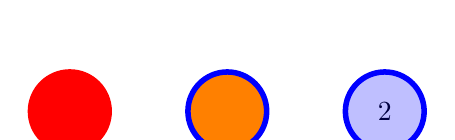
\begin{tikzpicture}[line width=2pt]
    \draw (2,0) node {$1$} (4,0) node {$2$};

    \filldraw[red]                    (0,0) circle (0.5);
    \filldraw[draw=blue,fill=orange]  (2,0) circle (0.5);
    \filldraw[blue,fill opacity=0.25] (4,0) circle (0.5);
\end{tikzpicture}
\end{verbbox}
\begin{center}
    $\vcenter{\hbox{
    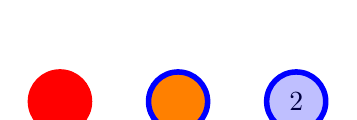
\begin{tikzpicture}[line width=2pt,scale=0.75]
        \draw (2,0) node {$1$} (4,0) node {$2$};

        \filldraw[red]                    (0,0) circle (0.5);
        \filldraw[draw=blue,fill=orange]  (2,0) circle (0.5);
        \filldraw[blue,fill opacity=0.25] (4,0) circle (0.5);
    \end{tikzpicture}
    }}$
    $\vcenter{\hbox{\theverbbox}}$
\end{center}



Sidenote on opacity and drawing precedence: \Tikz{} draws objects on top of each other, in the order they are given. So, if you want something to appear behind something else, the obscured object must be drawn first, i.e. above the line where the obscuring object is drawn.

As well as passing options to individual \verb|\draw| commands, you can pass options to the environment to set that option globally for everything in that environment. For instance, the \verb|line width| option for all the draw commands is set to \verb|2pt| at the top, so we don't need to set it for each draw command individually.

Stroke widths affect the width of the paths drawn, and can be set with. There are various built-in widths available:
\begin{verbbox}[\small\mbox{}]
    
\begin{tikzpicture}[yscale=0.4]
        \draw[ultra thin]  (0,6) -- (3,6);
        \draw[very thin]   (0,5) -- (3,5);
        \draw[thin]        (0,4) -- (3,4);
        \draw[semithick]   (0,3) -- (3,3);
        \draw[thick]       (0,2) -- (3,2);
        \draw[very thick]  (0,1) -- (3,1);
        \draw[ultra thick] (0,0) -- (3,0);
    \end{tikzpicture}
\end{verbbox}
\begin{center}
    $\vcenter{\hbox{
    
\begin{tikzpicture}[yscale=0.4]
        \draw[ultra thin]  (0,6) -- (3,6);
        \draw[very thin]   (0,5) -- (3,5);
        \draw[thin]        (0,4) -- (3,4);
        \draw[semithick]   (0,3) -- (3,3);
        \draw[thick]       (0,2) -- (3,2);
        \draw[very thick]  (0,1) -- (3,1);
        \draw[ultra thick] (0,0) -- (3,0);
    \end{tikzpicture}
    }}$
    $\vcenter{\hbox{\theverbbox}}$
\end{center}
Arrows can also be added using this syntax:
\begin{verbatim}
    \draw[->] ...
\end{verbatim}
or similar. There are also various types of arrowheads, \verb|>| being one of the basic kinds. More configurations are listed below (list is not exhaustive):
\begin{verbbox}[\small\mbox{}]
    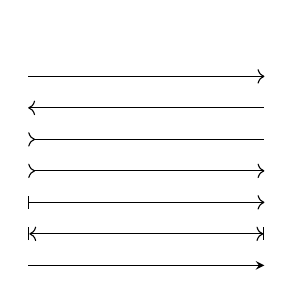
\begin{tikzpicture}[yscale=0.4]
        \draw[->]                   (0,7) -- (3,7);
        \draw[<-]                   (0,6) -- (3,6);
        \draw[>-]                   (0,5) -- (3,5);
        \draw[>->]                  (0,4) -- (3,4);
        \draw[|->]                  (0,3) -- (3,3);
        \draw[|<->|]                (0,2) -- (3,2);
        \draw[-stealth]             (0,1) -- (3,1);
        \draw[-latex]               (0,0) -- (3,0);
    \end{tikzpicture}
\end{verbbox}
\begin{center}
    $\vcenter{\hbox{
    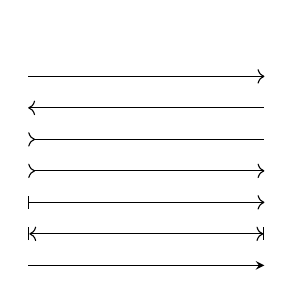
\begin{tikzpicture}[yscale=0.4]
        \draw[->]                   (0,7) -- (3,7);
        \draw[<-]                   (0,6) -- (3,6);
        \draw[>-]                   (0,5) -- (3,5);
        \draw[>->]                  (0,4) -- (3,4);
        \draw[|->]                  (0,3) -- (3,3);
        \draw[|<->|]                (0,2) -- (3,2);
        \draw[-stealth]             (0,1) -- (3,1);
        \draw[-latex]               (0,0) -- (3,0);
    \end{tikzpicture}
    }}$
    $\vcenter{\hbox{\theverbbox}}$
\end{center}
Other usual options may also be passed locally to the arrowhead:
\begin{verbbox}[\small\mbox{}]
    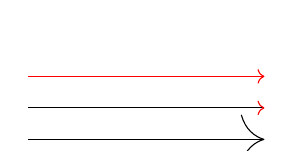
\begin{tikzpicture}[yscale=0.4]
        \draw[red,->]           (0,2) -- (3,2);
        \draw[-{>[red]}]        (0,1) -- (3,1);
        \draw[-{>[length=3mm]}] (0,0) -- (3,0);
    \end{tikzpicture}
\end{verbbox}
\begin{center}
    $\vcenter{\hbox{
    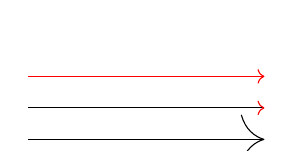
\begin{tikzpicture}[yscale=0.4]
        \draw[red,->]           (0,2) -- (3,2);
        \draw[-{>[red]}]        (0,1) -- (3,1);
        \draw[-{>[length=3mm]}] (0,0) -- (3,0);
    \end{tikzpicture}
    }}$
    $\vcenter{\hbox{\theverbbox}}$
\end{center}
Lines can also be dashed/dotted. There are various built-in patterns available (list is not exhaustive):
\begin{verbbox}[\small\mbox{}]
    \begin{tikzpicture}[yscale=0.4]
        \draw[dotted]         (0,6) -- (3,6);
        \draw[densely dotted] (0,5) -- (3,5);
        \draw[loosely dotted] (0,4) -- (3,4);
        \draw[dashed]         (0,3) -- (3,3);
        \draw[densely dashed] (0,2) -- (3,2);
        \draw[loosely dashed] (0,1) -- (3,1);
        \draw[dash dot]       (0,0) -- (3,0);
    \end{tikzpicture}
\end{verbbox}
\begin{center}
    $\vcenter{\hbox{
    \begin{tikzpicture}[yscale=0.4]
        \draw[dotted]         (0,6) -- (3,6);
        \draw[densely dotted] (0,5) -- (3,5);
        \draw[loosely dotted] (0,4) -- (3,4);
        \draw[dashed]         (0,3) -- (3,3);
        \draw[densely dashed] (0,2) -- (3,2);
        \draw[loosely dashed] (0,1) -- (3,1);
        \draw[dash dot]       (0,0) -- (3,0);
    \end{tikzpicture}
    }}$
    $\vcenter{\hbox{\theverbbox}}$
\end{center}
More generally, you can specify the pattern manually using the \verb|dash pattern| option:
\begin{verbatim}
    dash pattern=x on y off
\end{verbatim}
where \verb|x| and \verb|y| are any \TeX{} dimensions.

Lines may also be \textit{decorated} as follows:
\begin{verbbox}[\small\mbox{}]
    \begin{tikzpicture}[decoration={
        markings,
        mark=at position 0.53 with {\arrow{>}}}
        ] 
        \draw[postaction={decorate}] (0,1) -- (3,1);
        \draw                        (0,0) -- (3,0);
    \end{tikzpicture}
\end{verbbox}
\begin{center}
    $\vcenter{\hbox{
    \begin{tikzpicture}[decoration={
        markings,
        mark=at position 0.53 with {\arrow{>}}}
        ] 
        \draw[postaction={decorate}] (0,1) -- (3,1);
        \draw                        (0,0) -- (3,0);
    \end{tikzpicture}
    }}$
    $\vcenter{\hbox{\theverbbox}}$
\end{center}
Note that arrow decorations are centred at their tips, so arrows need to be positioned slightly past the halfway point (e.g. 0.53 in the above) to appear properly centred.




\subsection*{Nodes}

Nodes are used to add text to a diagram. They may be specified and drawn using the following syntax:
\begin{verbatim}
    \node at (x,y) [options] {label}
\end{verbatim}
They may also be added to paths using the special path operation \verb|node|:
\begin{verbbox}[\small\mbox{}]
    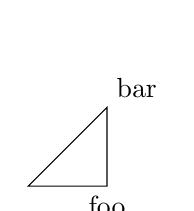
\begin{tikzpicture}
        \draw
            (0,0)
         -- (1,0) node [below]       {foo}
         -- (1,1) node [above right] {bar}
         -- cycle;
    \end{tikzpicture}
\end{verbbox}
\begin{center}
    $\vcenter{\hbox{
    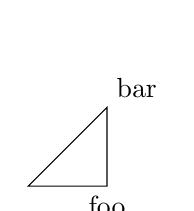
\begin{tikzpicture}
        \draw
            (0,0)
         -- (1,0) node [below]       {foo}
         -- (1,1) node [above right] {bar}
         -- cycle;
    \end{tikzpicture}
    }}$
    $\vcenter{\hbox{\theverbbox}}$
\end{center}
Nodes are specified in this way are positioned at the last coordinate mentioned. Note that nodes are specified in this way are also \textit{not} part of the path itself; they are separate elements drawn before or after the path:
\begin{verbbox}[\small\mbox{}]
    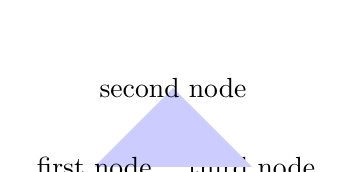
\begin{tikzpicture}[fill=blue!20!white]
    \fill
        (0,0) node               {first node}
     -- (1,1) node               {second node}
     -- (2,0) node [behind path] {third node};
    \end{tikzpicture}
\end{verbbox}
\begin{center}
    $\vcenter{\hbox{
    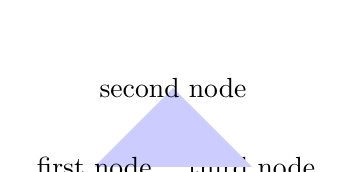
\begin{tikzpicture}[fill=blue!20!white]
    \fill
        (0,0) node               {first node}
     -- (1,1) node               {second node}
     -- (2,0) node [behind path] {third node};
    \end{tikzpicture}
    }}$
    $\vcenter{\hbox{\theverbbox}}$
\end{center}

Nodes may also be placed on paths by specifying the node after a path starts, but before the endpoint is specified:
\begin{verbbox}[\small\mbox{}]
    \begin{tikzpicture}
    \begin{tikzpicture}
    \draw
        (0,0) -- node {$p$}
        (1,1) node {$X$};
    \end{tikzpicture}
\end{verbbox}
\begin{center}
    $\vcenter{\hbox{
    \begin{tikzpicture}
    \draw
        (0,0) -- node {$p$}
        (1,1) node {$X$};
    \end{tikzpicture}
    }}$
    $\vcenter{\hbox{\theverbbox}}$
\end{center}

Nodes may also take some standard shapes as options (as well as colours, opacities, etc.). Passing the \verb|draw| option along with these shapes will draw the shape around the node, dynamically resizing to fit the label inside:
\begin{verbbox}[\small\mbox{}]
    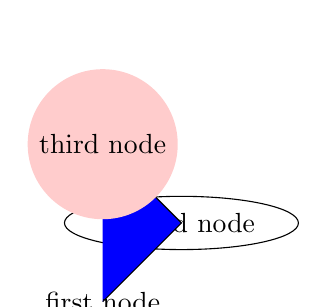
\begin{tikzpicture}
        \draw[fill=blue]
            (0,0) node                            {first node}
         -- (1,1) node[ellipse,draw, behind path] {second node}
         -- (0,2) node[circle,fill=red!20]        {third node};
        \end{tikzpicture}
\end{verbbox}
\begin{center}
    $\vcenter{\hbox{
    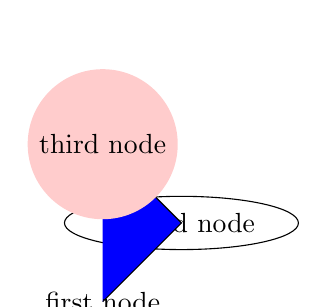
\begin{tikzpicture}
        \draw[fill=blue]
            (0,0) node                            {first node}
         -- (1,1) node[ellipse,draw, behind path] {second node}
         -- (0,2) node[circle,fill=red!20]        {third node};
    \end{tikzpicture}
    }}$
    $\vcenter{\hbox{\theverbbox}}$
\end{center}
Nodes may also be given names:
\begin{verbatim}
    \node (name) at (x,y) {label}
    \path ... -- (x,y) node (name) {label} -- ...
\end{verbatim}
A named node may be later referenced by its name. This is useful for computation on coordinates, etc.

% Nodes also naturally interoperate with \Tikz{}'s iteration system:





\subsection*{Coordinate Computation}
We have already seen some computation within coordinates, but we can do a lot more than simply adding dimensions together.

A coordinate computation is marked with a pair of \$ symbols. One basic computation is to add and scale coordinates:
\begin{verbbox}[\small\mbox{}]
    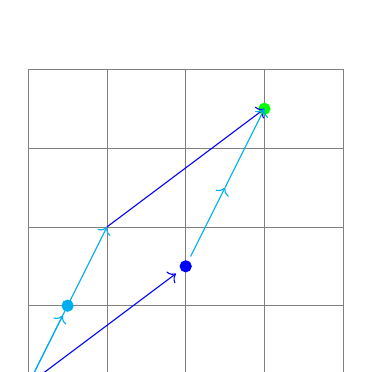
\begin{tikzpicture}
        \draw[help lines] (0,0) grid (4,4);
        
        \filldraw[blue] (2,1.5) circle (2pt) node (a) {};
        \filldraw[cyan] (0.5,1) circle (2pt) node (b) {};
        \filldraw[green] ($(a) + 2*(b)$) circle (2pt);

        \draw[blue,->] (0,0) -- (a);
        \draw[blue,->] ($2*(b)$) -- ($(a) + 2*(b)$);

        \draw[cyan,->] (0,0) -- (b);
        \draw[cyan,->] (0,0) -- ($2*(b)$);
        \draw[cyan,->] (a) -- ($(a) + (b)$);
        \draw[cyan,->] ($(a) + (b)$) -- ($(a) + 2*(b)$);
    \end{tikzpicture}
\end{verbbox}
\begin{center}
    $\vcenter{\hbox{
    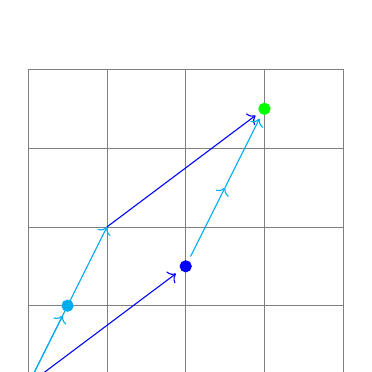
\begin{tikzpicture}
        \draw[help lines] (0,0) grid (4,4);
        
        \filldraw[blue] (2,1.5) circle (2pt) node (a) {};
        \filldraw[cyan] (0.5,1) circle (2pt) node (b) {};
        \filldraw[green] ($ (a) + 2*(b) $) circle (2pt);

        \draw[blue,->] (0,0) -- (a);
        \draw[blue,->,shorten >=4pt] ($2*(b)$) -- ($(a) + 2*(b)$);

        \draw[cyan,->] (0,0) -- (b);
        \draw[cyan,->] (0,0) -- ($2*(b)$);
        \draw[cyan,->] (a) -- ($(a) + (b)$);
        \draw[cyan,->,shorten >=4pt] ($(a) + (b)$) -- ($(a) + 2*(b)$);
    \end{tikzpicture}
    }}$
    $\vcenter{\hbox{\theverbbox}}$
\end{center}

A coordinate may be followed by various kinds of modifiers. The first kind of interest is the \textit{partway modifier}, with syntax:
\begin{verbatim}
    (a)!N!(b)
\end{verbatim}
The number \verb|N| linearly interpolates between the first and second coordinates:
\begin{equation*}
    (1-N)(a)+N(b)
\end{equation*}
Note that \verb|N| need not be between $0$ and $1$.

If \verb|N| instead has a dimension, e.g. \verb|N=1cm|, then this is the \textit{distance modifier}, and instead returns the point at distance \verb|N| from \verb|(a)| along the line connecting \verb|(a)| and \verb|(b)|.

If \verb|N| is instead itself is a coordinate, e.g. \verb|N=(c)|, then this is the \textit{projection modifier}, and instead returns the projection of \verb|N| on to the line connecting \verb|(a)| and \verb|(b)|.


\begin{verbbox}[\small\mbox{}]
    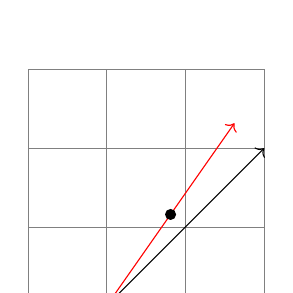
\begin{tikzpicture}
        \draw [help lines] (0,0) grid (3,3);
        \coordinate (a) at (1,0);
        \coordinate (b) at (3,2);

        \draw[->] (a) -- (b);
        \coordinate (c) at ($ (a)!1! 10:(b) $);
        \draw[->,red] (a) -- (c);
        \fill ($ (a)!.5! 10:(b) $) circle (2pt);
    \end{tikzpicture}
\end{verbbox}
\begin{center}
    $\vcenter{\hbox{
    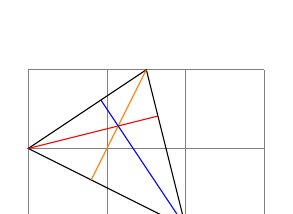
\begin{tikzpicture}
        \draw [help lines] (0,0) grid (3,2);
        
        \coordinate (a) at (0,1);
        \coordinate (b) at (1.5,2);
        \coordinate (c) at (2,0);
        
        \draw (a) -- (b) -- (c) -- cycle;
        
        \draw[red]    (a) -- ($(b)!(a)!(c)$);
        \draw[orange] (b) -- ($(a)!(b)!(c)$);
        \draw[blue]   (c) -- ($(a)!(c)!(b)$);
    \end{tikzpicture}
    }}$
    $\vcenter{\hbox{\theverbbox}}$
\end{center}
Another kind of modifier is the \textit{angle modifier}, with syntax:
\begin{verbatim}
    (a)!N!T:(b)
\end{verbatim}
(\verb|N| cannot be omitted from this; just set \verb|N=1| if the other modifiers are not desired.)

The number \verb|T| rotates the line from \verb|(a)| to \verb|(b)| about the point \verb|(a)| by \verb|T| degrees:

\begin{verbbox}[\small\mbox{}]
    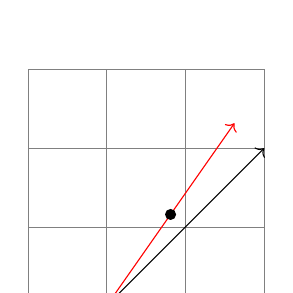
\begin{tikzpicture}
        \draw [help lines] (0,0) grid (3,3);
        \coordinate (a) at (1,0);
        \coordinate (b) at (3,2);

        \draw[->] (a) -- (b);
        \coordinate (c) at ($ (a)!1! 10:(b) $);
        \draw[->,red] (a) -- (c);
        \fill ($ (a)!.5! 10:(b) $) circle (2pt);
    \end{tikzpicture}
\end{verbbox}
\begin{center}
    $\vcenter{\hbox{
    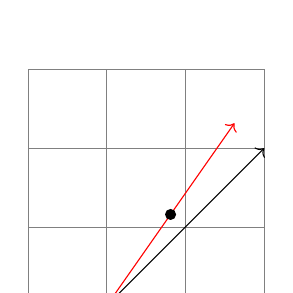
\begin{tikzpicture}
        \draw [help lines] (0,0) grid (3,3);
        \coordinate (a) at (1,0);
        \coordinate (b) at (3,2);
        
        \draw[->] (a) -- (b);
        \coordinate (c) at ($ (a)!1!10:(b) $);
        \draw[->,red] (a) -- (c);
        \fill ($ (a)!.5! 10:(b) $) circle (2pt);
    \end{tikzpicture}
    }}$
    $\vcenter{\hbox{\theverbbox}}$
\end{center}



\begin{verbbox}[\small\mbox{}]
    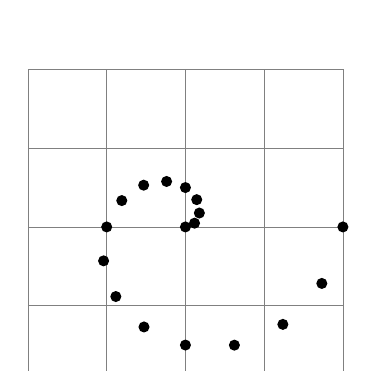
\begin{tikzpicture}
        \draw [help lines] (0,0) grid (4,4);
    
        \foreach \i in {0,0.125,...,2} {
            \fill ($(2,2) !\i! \i*180:(3,2)$) circle (2pt);
        }
    \end{tikzpicture}
\end{verbbox}
\begin{center}
    $\vcenter{\hbox{
    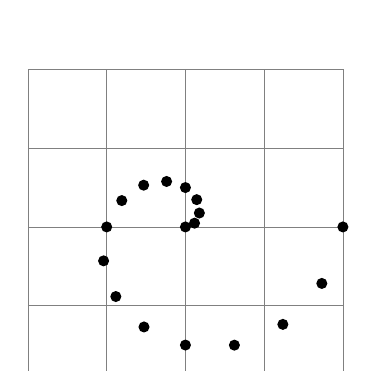
\begin{tikzpicture}
        \draw [help lines] (0,0) grid (4,4);
    
        \foreach \i in {0,0.125,...,2} {
            \fill ($(2,2) !\i! \i*180:(3,2)$) circle (2pt);
        }
    \end{tikzpicture}
    }}$
    $\vcenter{\hbox{\theverbbox}}$
\end{center}





\section*{Iteration}

\begin{tikzpicture}
    \foreach \x in {0,1,2,3} {
        \foreach \y in {0,1,2,3} {
            \filldraw (\x,\y) circle (2pt);
        }
    }
\end{tikzpicture}

\section*{Plots}

For small plots, you can use the special path operation \verb|plot|. This requires you to handle a lot of things manually, like adding axes/ticks, but is suitable for simplistic plots.

The \verb|plot| command can be used to connect a list of coordinates together:
\begin{verbbox}[\small\mbox{}]
    \begin{tikzpicture}
        \draw plot coordinates {(0,0) (1,1) (2,0) (3,1) (2,1) (10:2cm)};
    \end{tikzpicture}
\end{verbbox}
\begin{center}
    $\vcenter{\hbox{
    \begin{tikzpicture}
        \draw plot coordinates {(0,0) (1,1) (2,0) (3,1) (2,1) (10:2cm)};
    \end{tikzpicture}
    }}$
    $\vcenter{\hbox{\theverbbox}}$
\end{center}
This isn't very useful by itself, since we could have just specified a path and stroked it manually, but this command can also read coordinates from external files.

The \verb|plot| command can be used to plot a function parametrically by giving a coordinate in terms of the macro \verb|\x|:


\begin{verbbox}[\small\mbox{}]
    \begin{tikzpicture}[domain=0:4]
        \draw[very thin,color=gray] (-0.1,-1.1) grid (3.9,3.9);
      
        \draw[->] (-0.2,0) -- (4.2,0) node[right] {$x$};
        \draw[->] (0,-1.2) -- (0,4.2) node[above] {$f(x)$};
      
        \draw[color=red] 
            plot (\x,\x)             node[right] {$f(x)=x$};
        \draw[color=blue]  
            plot (\x,{sin(deg(\x))}) node[right] {$f(x) = \sin x$};
        \draw[color=orange]
            plot (\x,{0.05*exp(\x)}) node[right] {$f(x) = \frac{1}{20} \mathrm e^x$};
    \end{tikzpicture}
\end{verbbox}
\begin{center}
    $\vcenter{\hbox{
    \begin{tikzpicture}[domain=0:4]
        \draw[very thin,color=gray] (-0.1,-1.1) grid (3.9,3.9);
      
        \draw[->] (-0.2,0) -- (4.2,0) node[right] {$x$};
        \draw[->] (0,-1.2) -- (0,4.2) node[above] {$f(x)$};
      
        \draw[color=red] 
            plot (\x,\x)             node[right] {$f(x)=x$};
        \draw[color=blue]  
            plot (\x,{sin(deg(\x))}) node[right] {$f(x) = \sin x$};
        \draw[color=orange]
            plot (\x,{0.05*exp(\x)}) node[right] {$f(x) = \frac{1}{20} \mathrm e^x$};
    \end{tikzpicture}
    }}$
    $\vcenter{\hbox{\theverbbox}}$
\end{center}





% To perform computations on iteration variables, use \pgfmathsetmacro

% To perform computation in axis environments, you will have to use PGF commands, e.g. \verb|pgfplotsinvokeforeach| rather than \verb{\foreach}, as most Tikz commands will not work there.

\newpage


\section*{Axis Environment}


\subsection*{ColorBrewer}

\begin{align*}
    g_n(x)=\begin{cases}
        2nx&x\in[0,\frac{1}{2n})\\
        -2n\bigl(x-\frac{1}{n}\bigr)&x\in[\frac{1}{2n},\frac{1}{n})\\
        0&x\in[\frac{1}{n},1]\\
    \end{cases}\qquad\qquad
    h_n(x)=\begin{cases}
        2n^2x&x\in[0,\frac{1}{2n})\\
        -2n^2\bigl(x-\frac{1}{n}\bigr)&x\in[\frac{1}{2n},\frac{1}{n})\\
        0&x\in[\frac{1}{n},1]\\
    \end{cases}
\end{align*}
\begin{center}
    \begin{samepage}
        \resizebox*{5cm}{!}{% 
        \begin{tikzpicture}[declare function={
            func(\x,\n)=
                    (2*\n*\x) * and(0 <= \x, \x < (1/(2*\n)))
                    +
                    (-2*\n*(\x - (1/\n))) * and((1/(2*\n)) <= \x, \x <= (1/\n))
                    +
                    (0) * ((1/\n) <= \x);
            }]
            \begin{axis}[%
                axis x line=middle,
                axis y line=middle,
                xmin=-0.1,
                xmax=1.1,
                ymin=-0.1,
                ymax=1.1,
                samples=100,
                domain=0:1,
                cycle multi list={Blues-9}
                ]
                \addplot+[thick] {func(x,9)};
                \addplot+[thick] {func(x,8)};
                \addplot+[thick] {func(x,7)};
                \addplot+[thick] {func(x,6)};
                \addplot+[thick] {func(x,5)};
                \addplot+[thick] {func(x,4)};
                \addplot+[thick] {func(x,3)};
                \addplot+[thick] {func(x,2)};
                \addplot+[thick] {func(x,1)};
            \end{axis}
        \end{tikzpicture}
    }%
    \qquad\qquad
    \resizebox*{5cm}{!}{% 
    \begin{tikzpicture}[declare function={
        func(\x,\n)=
                (2*(\n^2)*\x) * and(0 <= \x, \x < (1/(2*\n)))
                +
                (-2*(\n^2)*(\x - (1/\n))) * and((1/(2*\n)) <= \x, \x <= (1/\n))
                +
                (0) * ((1/\n) <= \x);
        }]
        \begin{axis}[%
            axis x line=middle,
            axis y line=middle,
            xmin=-0.1,
            xmax=1.1,
            ymin=-1,
            ymax=11,
            samples=100,
            domain=0:1,
            cycle multi list={Blues-9}
            ]
            \addplot+[thick] {func(x,9)};
            \addplot+[thick] {func(x,8)};
            \addplot+[thick] {func(x,7)};
            \addplot+[thick] {func(x,6)};
            \addplot+[thick] {func(x,5)};
            \addplot+[thick] {func(x,4)};
            \addplot+[thick] {func(x,3)};
            \addplot+[thick] {func(x,2)};
            \addplot+[thick] {func(x,1)};
        \end{axis}
    \end{tikzpicture}
}%
\end{samepage}
\end{center}






% \section*{Your First \Tikz{} Diagram}






\newpage
\section*{Anchors}

\tikzset{
    shape example/.style= {color = black!30,
                           draw,
                           fill = yellow!30,
                           line width = .5cm,
                           inner xsep = 2.5cm,
                           inner ysep = 0.5cm}
}

\begin{center}
    \begin{tikzpicture}
        \node[name=s,shape=circle,shape example] {Circle\vrule width 1pt height 2cm};
        \foreach \anchor/\placement in
            {north west/above left, north/above, north east/above right,
            west/left, center/above, east/right,
            mid west/right, mid/above, mid east/left,
            base west/left, base/below, base east/right,
            south west/below left, south/below, south east/below right,
            text/left, 10/right, 130/above}
            \draw[shift=(s.\anchor)] plot[mark=x] coordinates{(0,0)}
                node[\placement] {\scriptsize\texttt{(s.\anchor)}};
    \end{tikzpicture}
\end{center}


\vspace*{2cm}

\begin{center}
    \begin{tikzpicture}
        \node[name=s,shape=rectangle,shape example] {Rectangle\vrule width 1pt height 2cm};
        \foreach \anchor/\placement in
            {north west/above left, north/above, north east/above right,
            west/left, center/above, east/right,
            mid west/right, mid/above, mid east/left,
            base west/left, base/below, base east/right,
            south west/below left, south/below, south east/below right,
            text/left, 10/right, 130/above}
            \draw[shift=(s.\anchor)] plot[mark=x] coordinates{(0,0)}
                node[\placement] {\scriptsize\texttt{(s.\anchor)}};
    \end{tikzpicture}
\end{center}




\newpage
\section*{Exercises}


\begin{enumerate}
    \item Recreate the following diagram:
    \begin{equation*}
        \Pi=\bigl\{\textcolor{blue}{x_1}=(1,0),{\textcolor{cyan}{x_2}}=(-1,1)\bigr\}
    \end{equation*}
    \begin{center}
        \begin{tikzpicture}[scale=2]
            \filldraw (0,0) circle (0.75pt);
            \draw[->, thick, blue] (0,0) -- (1,0)  node[right]      {$\textcolor{blue}{x_1}$};
            \draw[->, thick, cyan] (0,0) -- (-1,1) node[above left] {$\textcolor{cyan}{x_2}$};
            \draw[->] (0,0) -- (1,1)   node[above right] {$2\textcolor{blue}{x_1}+\textcolor{cyan}{x_2}$};
            \draw[->] (0,0) -- (0,1)   node[above]       {$\textcolor{blue}{x_1}+\textcolor{cyan}{x_2}$};
            \draw[->] (0,0) -- (-1,0)  node[left]        {$-\textcolor{blue}{x_1}$};
            \draw[->] (0,0) -- (-1,-1) node[below left]  {$-2\textcolor{blue}{x_1}-\textcolor{cyan}{x_2}$};
            \draw[->] (0,0) -- (0,-1)  node[below]       {$-\textcolor{blue}{x_1}-\textcolor{cyan}{x_2}$};
            \draw[->] (0,0) -- (1,-1)  node[below right] {$-\textcolor{cyan}{x_2}$};
        \end{tikzpicture}
    \end{center}

    \item Recreate the following diagrams:
    \begin{center}
        \scalebox{1.25}{
        \begin{tikzpicture}[scale=0.5,baseline={(0,0)},decoration={
                markings,
                mark=at position 0.53 with {\arrow{>}}}
                ]
            \draw[->] (-2,0) -- (2,0) node [right] {$x_0$};
            \filldraw (0,0) circle (2pt);
            \draw (0,-2) node {$\Delta^0$};
        \end{tikzpicture}
        \qquad
        \begin{tikzpicture}[scale=0.5,baseline={(0,0)},decoration={
                markings,
                mark=at position 0.53 with {\arrow{>}}}
                ]
            \draw[->] (-1,0) -- (3,0) node [right] {$x_0$};
            \draw[->] (0,-1) -- (0,3) node [above] {$x_1$};
            \filldraw (1,0) circle (2pt) -- (0,1) circle (2pt);
            \draw (0,-2) node {$\Delta^1$};
        \end{tikzpicture}
        \qquad
        \begin{tikzpicture}[scale=0.5,baseline={(0,0)},decoration={
                markings,
                mark=at position 0.53 with {\arrow{>}}}
                ]
            \draw[->] (-1,0) -- (3,0) node [right] {$x_0$};
            \draw[->] (0,-1) -- (0,3) node [above] {$x_1$};
            \draw[->] (-0.75,-0.75) -- (2.25,2.25) node [above right] {$x_2$};
            \filldraw[color=red!50, opacity=0.75] (1,0) -- (0,1) -- (0.75,0.75) -- cycle;
            \filldraw (1,0) circle (2pt) -- (0,1) circle (2pt) -- (0.75,0.75) circle (2pt) -- (1,0);
            \draw (0,-2) node {$\Delta^2$};
        \end{tikzpicture}
        }
    \end{center}

    \item Recreate the following diagram:
    \begin{center}
        \begin{tikzpicture}[scale=6]
            \coordinate (001) at (0,0);
            \coordinate (010) at (0.5,0.866);
            \coordinate (100) at (1,0);
            \coordinate (011) at ($ 1/2*(001) + 1/2*(010) $);
            \coordinate (101) at ($ 1/2*(001) + 1/2*(100) $);
            \coordinate (110) at ($ 1/2*(010) + 1/2*(100) $);
            \coordinate (111) at ($ 1/3*(001) + 1/3*(010) + 1/3*(100)$);

            \filldraw (001) circle (0.25pt) node [below left]  {$(0,0,1)$};
            \filldraw (010) circle (0.25pt) node [above]       {$(0,1,0)$};
            \filldraw (100) circle (0.25pt) node [below right] {$(1,0,0)$};
            \filldraw (011) circle (0.25pt) node [above left]  {$(0,1,1)$};
            \filldraw (101) circle (0.25pt) node [below]       {$(1,0,1)$};
            \filldraw (110) circle (0.25pt) node [above right] {$(1,1,0)$};
            \filldraw (111) circle (0.25pt) node [right]       {$(1,1,1)$};

            \begin{scope}[on background layer]
                \draw[thick, red]     (001) -- (010);
                \draw[thick, blue]    (010) -- (100);
                \draw[thick, green]   (100) -- (001);
                \draw[thick, cyan]    (011) -- (100);
                \draw[thick, magenta] (101) -- (010);
                \draw[thick, yellow]  (110) -- (001);
                \draw[thick] (111) circle (0.289);
            \end{scope}
        \end{tikzpicture}
    \end{center}

    \item Recreate (some of) the following diagrams:
    \begin{center}
        \begin{tikzpicture}[baseline=(base)]
            \begin{axis}[
                width=5cm,
                height=5cm,
                xmin=-1,
                xmax=1,
                ymin=-1,
                ymax=1,
                axis x line=center,
                axis y line=center,
                xticklabels={},
                yticklabels={},
                xlabel={$x$},
                ylabel={$f(x)$},
                xlabel style={right},
                ylabel style={above}
                ]
                \draw (0, 0) [color = red] circle [radius=0pt]coordinate(base);
                \addplot[thick, domain=-1:1, samples=100, red] {(1/3)*tan(deg(x))+(1/4)};
            \end{axis}
        \end{tikzpicture}
        \begin{tikzpicture}[baseline=(base)]
            \begin{axis}[
            width=2cm,
            height=5cm,
            xmin=-1,
            xmax=1,
            ymin=-1,
            ymax=1,
            xlabel={},
            ylabel={},
            xticklabels={},
            yticklabels={},
            axis line style={draw=none},
            tick style={draw=none},
            ]
                \draw (0, 0) [color = red] circle [radius=0pt]coordinate(base);
                \draw [black] (axis cs:0,0) circle (0pt) node {$+$};
            \end{axis}
        \end{tikzpicture}
        \begin{tikzpicture}[baseline=(base)]
            \begin{axis}[
                width=5cm,
                height=5cm,
                xmin=-1,
                xmax=1,
                ymin=-1,
                ymax=1,
                axis x line=center,
                axis y line=center,
                xticklabels={},
                yticklabels={},
                xlabel={$x$},
                ylabel={$g(x)$},
                xlabel style={right},
                ylabel style={above}
                ]
                \draw (0, 0) [color = red] circle [radius=0pt]coordinate(base);
                \addplot[thick, domain=-1:1, samples=100, blue] {-x^3-(1/5)*x^2+(1/2)*x};
            \end{axis}
        \end{tikzpicture}
        \begin{tikzpicture}[baseline=(base)]
            \begin{axis}[
            width=2cm,
            height=5cm,
            xmin=-1,
            xmax=1,
            ymin=-1,
            ymax=1,
            xlabel={},
            ylabel={},
            xticklabels={},
            yticklabels={},
            axis line style={draw=none},
            tick style={draw=none},
            ]
                \draw (0, 0) [color = red] circle [radius=0pt]coordinate(base);
                \draw [black] (axis cs:0,0) circle (0pt) node {$=$};
            \end{axis}
        \end{tikzpicture}
        \begin{tikzpicture}[baseline=(base)]
            \begin{axis}[
                width=5cm,
                height=5cm,
                xmin=-1,
                xmax=1,
                ymin=-1,
                ymax=1,
                axis x line=center,
                axis y line=center,
                xticklabels={},
                yticklabels={},
                xlabel={$x$},
                ylabel={$(f+g)(x)$},
                xlabel style={right},
                ylabel style={above}
                ]
                \draw (0, 0) [color = red] circle [radius=0pt]coordinate(base);
                \addplot[thin, dashed, domain=-1:1, samples=100, red] {(1/3)*tan(deg(x))+(1/4)};
                \addplot[thin, dashed, domain=-1:1, samples=100, blue] {-x^3-(1/5)*x^2+(1/2)*x};
                \addplot[thick, domain=-1:1, samples=100, green] {(1/3)*tan(deg(x))+(1/4)-x^3-(1/5)*x^2+(1/2)*x};
            \end{axis}
        \end{tikzpicture}
    \end{center}
    \begin{center}
        \begin{tikzpicture}[baseline=(base)]
            \begin{axis}[
                width=2cm,
                height=5cm,
                xmin=-1,
                xmax=1,
                ymin=-1,
                ymax=1,
                xlabel={},
                ylabel={},
                xticklabels={},
                yticklabels={},
                axis line style={draw=none},
                tick style={draw=none},
                ]
                \coordinate (base) at (0,0);
                \draw [black] (axis cs:0,0) circle (0pt) node {$2$};
            \end{axis}
        \end{tikzpicture}
        \begin{tikzpicture}[baseline=(base)]
            \begin{axis}[
                width=5cm,
                height=5cm,
                xmin=-1,
                xmax=1,
                ymin=-1,
                ymax=1,
                axis x line=center,
                axis y line=center,
                xticklabels={},
                yticklabels={},
                xlabel={$x$},
                ylabel={$f(x)$},
                xlabel style={right},
                ylabel style={above}
                ]
                \coordinate (base) at (0,0);
                \addplot[thick, domain=-1:1, samples=100, red] {(exp(-x^2)/4)*cos(10*deg(x))};
            \end{axis}
        \end{tikzpicture}
        \begin{tikzpicture}[baseline=(base)]
            \begin{axis}[
                width=2cm,
                height=5cm,
                xmin=-1,
                xmax=1,
                ymin=-1,
                ymax=1,
                xlabel={},
                ylabel={},
                xticklabels={},
                yticklabels={},
                axis line style={draw=none},
                tick style={draw=none},
                ]
                \coordinate (base) at (0,0);
                \draw [black] (axis cs:0,0) circle (0pt) node {$=$};
            \end{axis}
        \end{tikzpicture}
        \begin{tikzpicture}[baseline=(base)]
            \begin{axis}[
                width=5cm,
                height=5cm,
                xmin=-1,
                xmax=1,
                ymin=-1,
                ymax=1,
                axis x line=center,
                axis y line=center,
                xticklabels={},
                yticklabels={},
                xlabel={$x$},
                ylabel={$(2f)(x)$},
                xlabel style={right},
                ylabel style={above}
                ]
                \coordinate (base) at (0,0);
                \addplot[thin, dashed, domain=-1:1, samples=100, red] {(exp(-x^2)/4)*cos(10*deg(x))};
                \addplot[thick, domain=-1:1, samples=100, green] {(exp(-x^2)/2)*cos(10*deg(x))};
            \end{axis}
        \end{tikzpicture}
    \end{center}

    \item Recreate (some of) the following diagrams:
    \begin{center}
        \begin{tikzpicture}
            \begin{axis}[
                width=5cm,
                height=5cm,
                xmin=-10,
                xmax=10,
                ymin=-0.5,
                ymax=1.5,
                axis x line=center,
                axis y line=center,
                ytick distance=0.5,
                xlabel={$x$},
                ylabel={$f(x)$},
                ]
                \addplot[thick, domain=-10:-0.25, samples=50, red] {sin(deg(x))/x};
                \addplot[thick, domain=0.25:10, samples=50, red] {sin(deg(x))/x};
                \draw [thick,red,fill opacity=0] (axis cs:0,1) circle (2pt) node {};
            \end{axis}
        \end{tikzpicture}
        \qquad
        \begin{tikzpicture}
            \begin{axis}[
                width=5cm,
                height=5cm,
                xmin=-2,
                xmax=2,
                ymin=-2,
                ymax=2,
                axis x line=center,
                axis y line=center,
                xtick distance=1,
                ytick distance=1,
                xlabel={$x$},
                ylabel={$g(x)$},
                ]
                \addplot[thick, domain=-2:1, samples=20, green] {-1};
                \addplot[thick, domain=1:2, samples=20, green] {1};
                \draw [thick,green,fill=white] (axis cs:1,-1) circle (2pt) node {};
                \draw [thick,green,fill=green] (axis cs:1,1) circle (2pt) node {};
            \end{axis}
        \end{tikzpicture}
        \qquad
        \begin{tikzpicture}
            \begin{axis}[
                width=5cm,
                height=5cm,
                xmin=-2,
                xmax=2,
                ymin=-2,
                ymax=2,
                axis x line=center,
                axis y line=center,
                xlabel={$x$},
                ylabel={$h(x)$},
                ]
                \addplot[thick, domain=-0.5:0.5, samples=1000, blue] {sin(deg(1/x))};
                \addplot[thick, domain=-2:-0.5, samples=50, blue] {sin(deg(1/x))};
                \addplot[thick, domain=0.5:2, samples=50, blue] {sin(deg(1/x))};
            \end{axis}
        \end{tikzpicture}
    \end{center}
    \vspace*{-0.25cm}
    \begin{align*}
        \mathclap{f(x)=\frac{\sin(x)}{x}}
        \hspace{5cm}
        \mathclap{g(x)=\begin{cases}
            -1&x<1\\
            1&x\geq1
        \end{cases}}
        \hspace{5cm}
        \mathclap{h(x)=\sin\left(\frac{1}{x}\right)}
    \end{align*}

    \item Recreate the following diagram:
    \begin{center}
        \begin{tikzpicture}[scale=2,baseline={(0,0)}]
            \draw (0,0) -- (1,0) -- (1,1) -- (0,1) -- (0,0);
            \draw[->]  (0,0.50) -- (0,0.49);
            \draw[->]  (1,0.50) -- (1,0.51);
            \draw[->>] (0.50,0) -- (0.55,0);
            \draw[->>] (0.50,1) -- (0.45,1);
            \filldraw[black] (0,0) circle (0.5pt) node [below left] {$p$};
            \filldraw[black] (1,0) circle (0.5pt) node [below right] {$q$};
            \filldraw[black] (0,1) circle (0.5pt) node [above left] {$q$};
            \filldraw[black] (1,1) circle (0.5pt) node [above right] {$p$};
    
            \filldraw[black] (0,0.5) circle (0pt) node [left] {$a$};
            \filldraw[black] (1,0.5) circle (0pt) node [right] {$a$};
            \filldraw[black] (0.5,0) circle (0pt) node [below] {$b$};
            \filldraw[black] (0.5,1) circle (0pt) node [above] {$b$};
    
            \draw (0.5,-0.4) node {$\mathbb{RP}^2$};
        \end{tikzpicture}
        \quad
        \begin{tikzpicture}[scale=2,baseline={(0,0)}]
            \filldraw[black] (0.5,0.5) node {$\cong$};
        \end{tikzpicture}
        \quad
        \begin{tikzpicture}[decoration={
                markings,
                mark=at position 0.53 with {\arrow{>}}},baseline={(0,-1)}
                ] 
            \draw[postaction={decorate}] (1,0) arc (0:180:1);
            \draw[postaction={decorate}] (-1,0) arc (180:360:1);
            \filldraw (1,0) circle (1pt) node [right] {$q$};
            \filldraw (-1,0) circle (1pt) node [left] {$q$};
            \draw (0,1) node [above] {$v$};
            \draw (0,-1) node [below] {$v$};
            \draw (0,-1.5) node {$v=a+b$};
        \end{tikzpicture}
        \qquad
        \begin{tikzpicture}[scale=2,baseline={(0,0)},decoration={
                markings,
                mark=at position 0.53 with {\arrow{>}}},baseline={(0,-1)}
                ] 
            \filldraw[dashed, fill=red, opacity=0.5] (0.0,0) circle (0.5);
            \filldraw[dashed, fill=white] (0.0,0) circle (0.3);
            \filldraw[dashed, fill=blue, opacity=0.5] (0.0,0) circle (0.4);
            \draw[postaction={decorate}] (0.5,0) arc (0:180:0.5);
            \draw[postaction={decorate}] (-0.5,0) arc (180:360:0.5);
            \filldraw (0.5,0) circle (0.5pt);
            \filldraw (-0.5,0) circle (0.5pt);
            \draw (0,-0.75) node {$\mathbb{RP}^2\subseteq\textcolor{red}{U}\cup\textcolor{blue}{V}$};
        \end{tikzpicture}
        \qquad
        \begin{tikzpicture}[scale=2,baseline={(0,0)},decoration={
            markings,
            mark=at position 0.53 with {\arrow{>}}},baseline={(0,-1)}
            ] 
        \filldraw[dashed, fill=red, opacity=0.5] (0.0,0) circle (0.4);
        \filldraw[dashed, fill=blue, opacity=0.5] (0.0,0) circle (0.4);
        \filldraw[dashed, fill=white] (0.0,0) circle (0.3);
        \draw (0,-0.75) node {$\textcolor{red}{U}\textcolor{red!50!blue}{\cap}\textcolor{blue}{V}$};
        \end{tikzpicture}
    \end{center}

    \item Recreate the following diagram:
    \begin{equation*}
        f_n(x)=\begin{cases}
            0 & 0\leq x<\frac{1}{2}-\frac{1}{n}\\
            1-n(\frac{1}{2}-x) & \frac{1}{2}-\frac{1}{n}\leq x<\frac{1}{2}\\
            1 & \frac{1}{2}<x\leq 1
        \end{cases}
    \end{equation*}
    \begin{center} 
        \begin{tikzpicture}[declare function={
            func(\x,\n)=
                    (0) * and(0 <= \x, \x < ((1/2) - (1/\n)))
                    +
                    (1 - \n*((1/2) - \x)) * and(((1/2) - (1/\n)) <= \x, \x <= (1/2))
                    +
                    (1) * ((1/2) < \x);
            }]
            \begin{axis}[%
                axis x line=middle,
                axis y line=middle,
                xmin=-0.1,
                xmax=1.1,
                ymin=-0.1,
                ymax=1.1,
                samples=500,
                domain=0:1,
                cycle multi list={Blues-9}
                ]
                \foreach \i in {2,...,10} {
                    \addplot+[thick] {func(x,\i)};
                }
            \end{axis}
        \end{tikzpicture}
    \end{center}
\end{enumerate}




\newpage
\section*{Samples}

\begin{center}
    \begin{tikzpicture}[baseline=(base)]
        \begin{axis}[
        width=6cm,
        height=5cm,
        xmin=-1,
        xmax=5,
        ymin=-1,
        ymax=4,
        axis x line=center,
        axis y line=center,
        xlabel={},
        ylabel={},
        grid=both,
        minor tick num=1,
        xtick distance=1,
        ytick distance=1,
        grid style={line width=.1pt, draw=gray!10},
        xticklabels={},
        yticklabels={},
        ]
            \draw (0, 0) [color = red] circle [radius=0pt]coordinate(base);
            \draw [very thin, draw=black, fill=lime, opacity=0.2] (axis cs:0,0) -- (axis cs:3,0) -- (axis cs:3,1) -- cycle;
            \draw [very thin, draw=black, fill=lime, opacity=0.2] (axis cs:1,2) -- (axis cs:4,3) -- (axis cs:1,3) -- cycle;
            \draw [very thin, draw=black, fill=teal, opacity=0.2] (axis cs:0,0) -- (axis cs:1,2) -- (axis cs:0,2) -- cycle;
            \draw [very thin, draw=black, fill=teal, opacity=0.2] (axis cs:3,1) -- (axis cs:4,1) -- (axis cs:4,3) -- cycle;
            \draw [very thin, draw=black, fill=red, opacity=0.2] (axis cs:3,0) -- (axis cs:4,0) -- (axis cs:4,1) -- (axis cs: 3,1) -- cycle;
            \draw [very thin, draw=black, fill=red, opacity=0.2] (axis cs:0,2) -- (axis cs:1,2) -- (axis cs:1,3) -- (axis cs: 0,3) -- cycle;
            \draw [very thin, draw=red, fill=yellow, opacity=0.2] (axis cs:0,0) -- (axis cs:3,1) -- (axis cs:4,3) -- (axis cs:1,2) -- cycle;
            \draw [->,blue,ultra thick] (axis cs:0,0) to (axis cs:3,1);
            \draw [->,cyan,ultra thick] (axis cs:0,0) to (axis cs:1,2);

            \draw [decorate,decoration={calligraphic brace,raise=1pt}] (axis cs:3,0) -- (axis cs:0,0)
            node[pos=0.5,below=2pt,black]{$\textcolor{blue}{a}$};
            
            \draw [decorate,decoration={calligraphic brace,raise=1pt}] (axis cs:4,0) -- (axis cs:3,0)
            node[pos=0.5,below=2pt,black]{$\textcolor{cyan}{b}$};

            \draw [decorate,decoration={calligraphic brace,raise=1pt}] (axis cs:0,3) -- (axis cs:1,3)
            node[pos=0.5,above=2pt,black]{$\textcolor{cyan}{b}$};
            
            \draw [decorate,decoration={calligraphic brace,raise=1pt}] (axis cs:1,3) -- (axis cs:4,3)
            node[pos=0.5,above=2pt,black]{$\textcolor{blue}{a}$};
            
            \draw [decorate,decoration={calligraphic brace,raise=1pt}] (axis cs:0,0) -- (axis cs:0,2)
            node[pos=0.5,left=2pt,black]{$\textcolor{cyan}{d}$};

            \draw [decorate,decoration={calligraphic brace,raise=1pt}] (axis cs:0,2) -- (axis cs:0,3)
            node[pos=0.5,left=2pt,black]{$\textcolor{blue}{c}$};
            
            \draw [decorate,decoration={calligraphic brace,raise=1pt}] (axis cs:4,3) -- (axis cs:4,1)
            node[pos=0.5,right=2pt,black]{$\textcolor{cyan}{d}$};

            \draw [decorate,decoration={calligraphic brace,raise=1pt}] (axis cs:4,1) -- (axis cs:4,0)
            node[pos=0.5,right=2pt,black]{$\textcolor{blue}{c}$};

            \draw [black] (axis cs:2.5,0.4) circle (0pt) node {$\textcolor{green!70!black}{\frac{ac}{2}}$};
            \draw [black] (axis cs:1.5,2.6) circle (0pt) node {$\textcolor{green!70!black}{\frac{ac}{2}}$};
            \draw [black] (axis cs:0.4,1.5) circle (0pt) node {$\textcolor{cyan!70!blue}{\frac{bd}{2}}$};
            \draw [black] (axis cs:3.6,1.5) circle (0pt) node {$\textcolor{cyan!70!blue}{\frac{bd}{2}}$};
            \draw [black] (axis cs:3.5,0.5) circle (0pt) node {$\textcolor{red}{bc}$};
            \draw [black] (axis cs:0.5,2.5) circle (0pt) node {$\textcolor{red}{bc}$};
        \end{axis}
    \end{tikzpicture}
\end{center}
\begin{equation*}
    \textcolor{yellow!70!orange}{\det\biggl[}\begin{matrix}
        \textcolor{blue}{a} & \textcolor{cyan}{b} \\
        \textcolor{blue}{c} & \textcolor{cyan}{d}
    \end{matrix}\textcolor{yellow!70!orange}{\biggr]}=(\textcolor{blue}{a}+\textcolor{cyan}{b})(\textcolor{blue}{c}+\textcolor{cyan}{d})-2\left(\textcolor{green!70!black}{\frac{ac}{2}}\right)-2\left(\textcolor{cyan!70!blue}{\frac{bd}{2}}\right)-2\textcolor{red}{bc}=\textcolor{blue}{a}\textcolor{cyan}{d}-\textcolor{cyan}{b}\textcolor{blue}{c}
\end{equation*}


\subsection*{Iteration}

\begin{center}
    \begin{tikzpicture}
        \foreach \n in {1,...,100}
            \draw[thin] (1/\n,0) circle (1/\n);
        \draw (0,0) node [left] {$h$};
    \end{tikzpicture}
\end{center}

\vspace*{2cm}

\begin{center}
    \begin{tikzpicture}
        \foreach \l in {0,1,2} {
            \foreach \r in {0,1,2} {
                \draw (0,2\l) -- (2,2\r);
            }
            \filldraw (0,2\l) circle (1.5pt);
            \filldraw (2,2\l) circle (1.5pt);
        }
    \end{tikzpicture}
\end{center}

\vspace*{2cm}

\begin{equation*}
    Z=\{0\}\cup\textcolor{blue}{\{2^{-n}:n\in\mathbb{Z}^+\}}\cup\textcolor{cyan}{\{2^{-n}+2^{-n-m}:n,m\in\mathbb{Z}^+\}}
\end{equation*}

\begin{center}
    \begin{tikzpicture}[scale=6]
        \draw[->] (-0.25,0) -- (1,0) node[right] {$\mathbb{R}$};
        \foreach \n in {1,...,10} {
            \foreach \m in {1,...,10} {
                \draw[cyan, thin]
                    ({2^(-\n)+2^(-\n-\m)},{-0.1*((10-\n)/10)*((10-\m)/10)})
                 -- ({2^(-\n)+2^(-\n-\m)},{ 0.1*((10-\n)/10)*((10-\m)/10)});
            }
            \ifnum\n<4
                \draw[blue]
                    ({2^(-\n)},{-0.15*((10-\n)/10)})
                 -- ({2^(-\n)},{ 0.15*((10-\n)/10)})
                    node[black,above,scale=1] {$2^{-\n}$};
            \else
                \ifnum\n=5
                    \draw[blue]
                        ({2^(-\n)},{-0.15*((10-\n)/10)})
                     -- ({2^(-\n)},{ 0.15*((10-\n)/10)})
                        node[black,above,scale=1] {$\cdots$};
                \else
                    \draw[blue] 
                        ({2^(-\n)},{-0.15*((10-\n)/10)})
                     -- ({2^(-\n)},{ 0.15*((10-\n)/10)});
                \fi
            \fi
        }
        \filldraw (0,0) circle (0.25pt) node[above left] {$0$};
    \end{tikzpicture}
\end{center}

Simpler version without if/else clauses for labels:
\begin{center}
    \begin{tikzpicture}[scale=6]
        \draw[->] (-0.25,0) -- (1,0) node[right] {$\mathbb{R}$};
        \foreach \n in {1,...,10} {
            \foreach \m in {1,...,10} {
                \draw[cyan, thin]
                    ({2^(-\n)+2^(-\n-\m)},{-0.1*((10-\n)/10)*((10-\m)/10)})
                 -- ({2^(-\n)+2^(-\n-\m)},{ 0.1*((10-\n)/10)*((10-\m)/10)});
            }
            \draw[blue]
                ({2^(-\n)},{-0.15*((10-\n)/10)})
             -- ({2^(-\n)},{0.15*((10-\n)/10)});
        }
    \end{tikzpicture}
\end{center}



\subsection*{Calc Library}

\begin{center}
    \begin{tikzpicture}[scale = 2]
        \begin{scope}[every node/.style={circle, fill, draw, inner sep=0, minimum size=5pt}]
            \node[label=left:{$v_0$}]  (v0) at (0,1) {};
            \node[label=below:{$v_1$}] (v1) at (1,0) {};
            \node[label=above:{$v_2$}] (v2) at (2,3.6) {};
            \node[label=right:{$v_3$}] (v3) at (4.8,0.3) {};
        \end{scope}
        \begin{scope}[every node/.style={circle, fill, draw, inner sep=0, minimum size=2pt}]
            \node (b01) at ($ 1/2*(v0) + 1/2*(v1) $) {};
            \node (b02) at ($ 1/2*(v0) + 1/2*(v2) $) {};
            \node (b03) at ($ 1/2*(v0) + 1/2*(v3) $) {};
            \node (b12) at ($ 1/2*(v1) + 1/2*(v2) $) {};
            \node (b13) at ($ 1/2*(v1) + 1/2*(v3) $) {};
            \node (b23) at ($ 1/2*(v2) + 1/2*(v3) $) {};
        \end{scope}
        \begin{scope}[every node/.style={circle, fill, draw, inner sep=0, minimum size=4pt}]
            \node[label={[xshift=1.5pt,yshift=0.5pt]0:{$b_0$}}]
                (b0) at ($ 1/3*(b13) + 1/3*(b12) + 1/3*(b23) $) {};
            \node[label={[yshift=1pt]70:{$b_1$}}]
                (b1) at ($ 1/3*(b02) + 1/3*(b03) + 1/3*(b23) $) {};
            \node[label=below:{$b_2$}]
                (b2) at ($ 1/3*(b01) + 1/3*(b03) + 1/3*(b13) $) {};
            \node[label=above left:{$b_3$}]
                (b3) at ($ 1/3*(b01) + 1/3*(b02) + 1/3*(b12) $) {};
        \end{scope}
        \begin{scope}[on background layer]
            \draw[thick, dash pattern=on 2pt off 1pt]
                (v0) -- (v3);
            \draw[yellow, dash pattern=on 2pt off 1pt]
                (v0) -- (b23)
                (v2) -- (b03)
                (v3) -- (b02);
            \draw[green, dash pattern=on 2pt off 1pt]
                (v0) -- (b13)
                (v1) -- (b03)
                (v3) -- (b01);
            \draw[very thin, dash pattern=on 2pt off 1pt]
                (b01) -- (b23)
                (b02) -- (b13)
                (b03) -- (b12);
            \draw[red]
                (v0) -- (b12)
                (v1) -- (b02)
                (v2) -- (b01);
            \draw[blue]
                (v1) -- (b23)
                (v2) -- (b13)
                (v3) -- (b12);
            \draw
                (v0) -- (b0)
                (v1) -- (b1)
                (v2) -- (b2)
                (v3) -- (b3);
            \draw[thick]
                (v0) -- (v1)
                (v0) -- (v2)
                (v1) -- (v2)
                (v1) -- (v3)
                (v2) -- (v3)
                (v2) -- (v3);
        \end{scope}
        \filldraw
            ($ 1/8*(v0) + 1/8*(v1) + 1/8*(v2) + 1/8*(v3)
             + 1/8*(b0) + 1/8*(b1) + 1/8*(b2) + 1/8*(b3) $)
            circle (2.5pt) node [above left=5pt and -2pt] {$b$};
    \end{tikzpicture}
\end{center}











\end{document}